% This is a document using the University of Minnesota, Morris, Computer Science
% Senior Seminar modification of the ACM sig-alternate style.

\documentclass{sig-alternate}
\usepackage{color}
\usepackage{gensymb}
\usepackage[colorinlistoftodos]{todonotes}

\begin{document}

\conferenceinfo{UMM CSci Senior Seminar Conference, December 2017}{Morris, MN}

\title{Foveated Rendering in Virtual Reality}

\numberofauthors{1}

\author{
% The command \alignauthor (no curly braces needed) should
% precede each author name, affiliation/snail-mail address and
% e-mail address. Additionally, tag each line of
% affiliation/address with \affaddr, and tag the
% e-mail address with \email.
\alignauthor
Samuel A. Miller\\
	\affaddr{Division of Science and Mathematics}\\
	\affaddr{University of Minnesota, Morris}\\
	\affaddr{Morris, Minnesota, USA 56267}\\
	\email{mill5978@morris.umn.edu}
}

\maketitle
\begin{abstract}

%In Progress Abstract
The question addressed in this paper is how best to implement foveated rendering to reduce computational load when rendering three-dimensional environments in virtual reality. The main goal in designing one of these renderers is to provide an experience in which the user is unable to distinguish whether they are seeing environments that are using these optimizations or not. Ideally you should be able to implement this technology to render the same scene with the same impact on the user, yet with a fraction of the computing power previously necessary for the scene.
\end{abstract}

\keywords{foveated rendering, gaze tracking, multiresolutional displays, virtual reality}

\section{Introduction}
\label{sec:intro}

Outline Notes: This section will ideally begin with a hook and then lay down the various components involved in my paper (virtual reality, computing power constraints, gaze tracking, foveated rendering etc)~\cite{Patney:Towards,Guenter:Foveated,Swafford:User}. Also, after consulting with my adviser I have decided to dedicate a portion of this section to applications/future uses for foveated rendering. This will be put in the intro as I don't think it will have enough substance to stand on its own, however it is important to include and will serve the useful purpose of communicating the importance of this technology to my audience.  
Topics to introduce:
\begin{itemize}
\item Virtual reality
\item hardware constraints
\item Human-vision-based restrictions
\item eye tracking
\item current state of foveated rendering
\end{itemize}

\section{Background}
\label{sec:background}

Outline Notes: This section will need to catch my audience up to speed on all of the concepts necessary to truly understand what this technology is doing and why it is useful.
The sources used in this section are the background sources found in my bibliography: \textit{Image processing by the human eye~\cite{Thibos:Image}, User performance with gaze contingent multiresolutional displays~\cite{Swafford:User}, Latency Requirements for Foveated Rendering in Virtual Reality~\cite{Albert:Latency}}, etc.

\subsection{Human Vision Overview}
\label{sec:visionOverview}

\begin{figure}
\centering
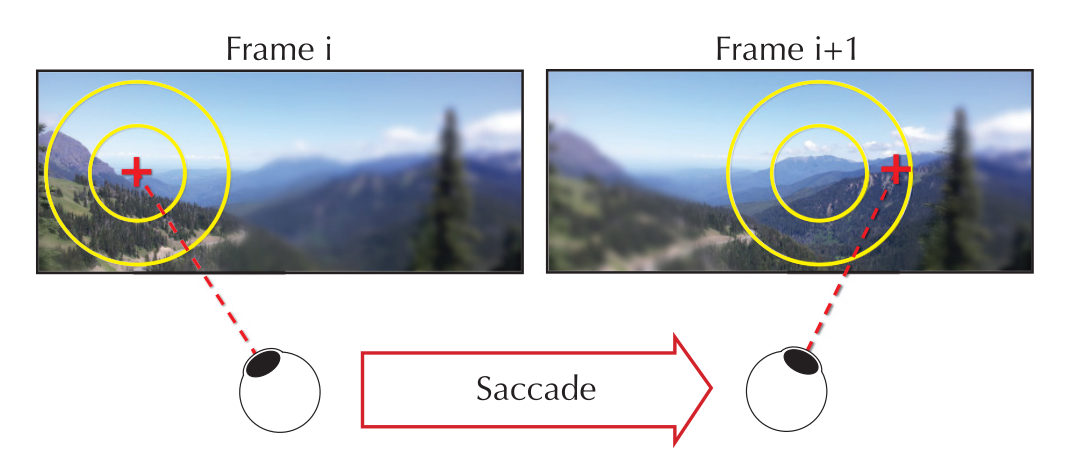
\psfig{file=saccade.png,width=3.5in}
\caption{Visualization of a saccadic eye movement from one foveated rendered frame to another.~\cite{Albert:Latency}}
\label{fig:fig1}
\end{figure}

Determining the strengths and weaknesses of the human eye is essential when developing technology that is primarily perceived visually. The key component of human vision that foveated rendering focuses on is the differences between fovea and periphery regions. The fovea is an area in the central region of vision approximately 5\degree~in diameter that contains the most spatial density of photorecptors in the eye, while the periphery is the surrounding area. A key difference in how these two regions are perceived is that the optic nerve undersamples the retinal image from the periphery, while all data gathered in the foveal region is not undersampled. This leads to the construction of a focal point, where changes perceived in the periphery will be noticeable, but not immediately identifiable.\cite{Guenter:Foveated, Thibos:Image}


Additional important visual concepts for this subject matter are that of \textit{retinal eccentricity} and \textit{saccadic eye movements}. 

Retinal eccentricity is the angular distance as you move away from the central focus of your vision~\cite{Guenter:Foveated}. \textit{Foveal layers}, the spatial divisions of regions which developers render at different resolutions, are based on retinal eccentricity by using it to dictate how large each region should be according to photoreceptor density on the retina.

Saccadic eye movements,(see \textbf{Figure~\ref{fig:fig1}}) are the simultaneous shift in focus of both eyes to a point that is a considerable distance from where they started. These movements are a critical weakness that foveated renderers must handle, as these movements are what make tracking the eye unpredictable. It is difficult to smoothly render a space based on the focal point of the eyeline if the user can shift his gaze somewhere else in an instant. Handling this weakness is one factor that held the advancement of this field back for so long, as latency proved to be an insurmountable restriction.
\subsection{Virtual Reality Headsets}
\label{sec:VRHMDs}

\begin{figure}
\centering
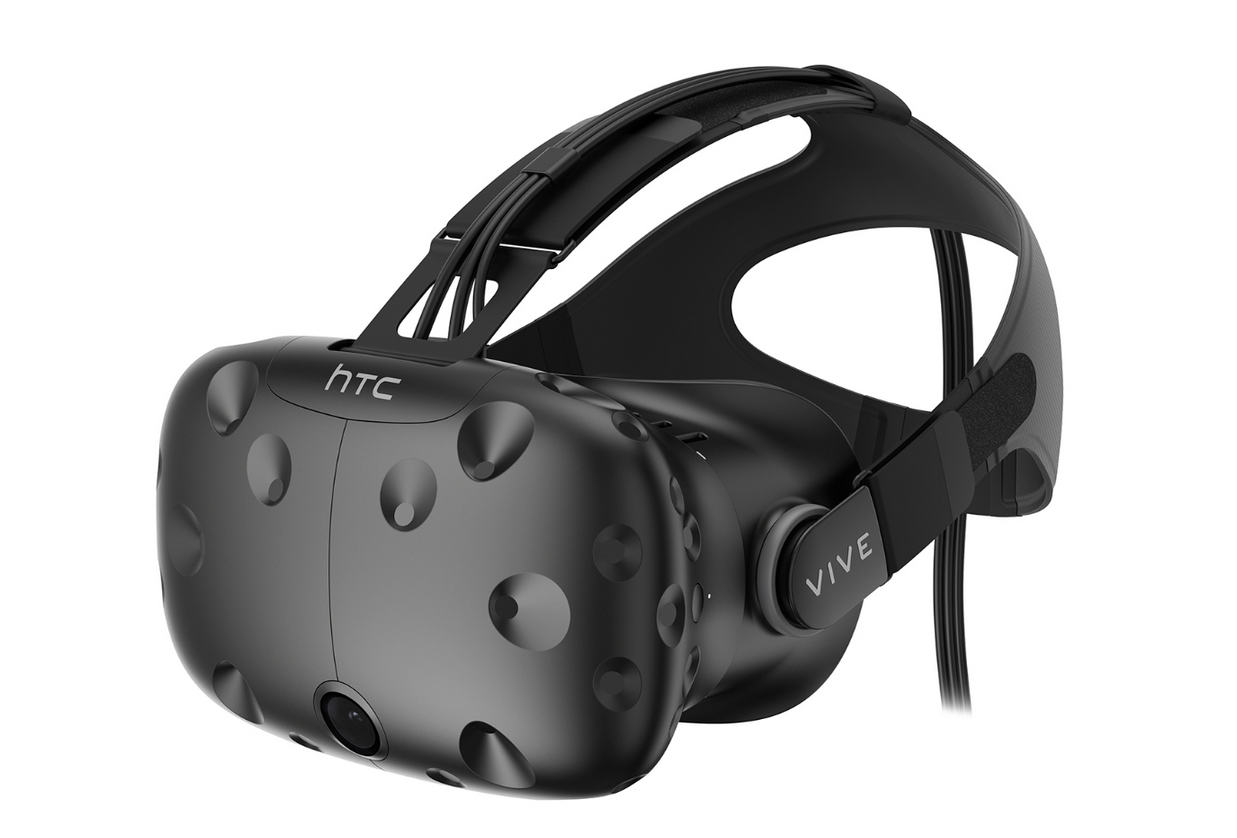
\psfig{file=vive.png,width =3in}
\caption{HTC Vive Virtual Reality Head Mounted Display.~\cite{Tom:derek}}
\label{fig:fig2}
\end{figure}



Virtual Reality (VR) displays have been a science fiction staple that developers have long tried to implement. There have been countless failures to make this technology feasible over the years, however it seems computing hardware has finally caught up. There has been a steadily increasing availability of affordable consumer options for VR, leading to a complementary increase in both public and corporate interest. This interest has yielded options for early adopters, such as the Oculus Rift and the HTC Vive, as well as the more casual consumer, such as Samsung's Gear VR and Google Carboard.

\todo[inline, color=white]{This section will range in brevity depending on if the previously mentioned products all need to be included/expanded upon or not. They all have relevancy but I think if I go into too much depth here this section may be the first to be cut down.}

While all of these options have their niche in the market, the scope of this paper will focus on the HMDs with the most computing power available to them, i.e. the HTC Vive (see \textbf{Figure~\ref{fig:fig2}}). The Vive targets a market that wants applications with complex scenes as well as high resolutions. It is devices like these that have an immediate demand for any avenue of optimization in order to meet the needs of their consumer base. These are the products that will adopt techniques like foveated rendering first.

\subsection{Gaze Tracking}
\label{sec:gazeTracking}

Gaze tracking is the practice of using a combination of hardware and software to compute the trajectory of the user's eyeline to determine what the center of their view is focused on. This technology has been used for a variety of purposes over the years, (i.e. interactible displays/accessibility services for those who are handicapped), and has now become increasingly in the public eye due to the commercial popularization of VR devices.

While gaze tracking hardware has been around for a suprisingly long time, it hasn't always been feasible for practical use. In 1990, Mark Levoy and Ross Whitaker explored ways of utilizing gaze tracking to develop rendering optimization algorithms. Their results showed promise, with their software responding to the gaze tracking well, however the subjects were placed in bulky headwear that limited the practicality of any similar implementation of foveated rendering. At the time, the setup demanded an NAC Eye Mark eye Tracker, (pictured in \textbf{Figure~\ref{fig:fig2}}), which covered a large portion of their head and had to be physically connected to rendering engine hardware. This hardware restriction left Levoy and Whitaker limited in what they could accomplish, as nearly the entire head was covered with technology purely devoted to gaze tracking. Integration with virtual reality would have been impossible at this time.~\cite{Levoy:Gaze}

However, gaze tracking has advanced drastically over the years. 2017 is a landmark year in that there are several implementations being released for public purchase. ``aGlass'', developed by 7invensun from Beijing, is an affordable modular upgrade to the HTC Vive that will be available for purchase later in 2017. This product is notable in that it will be able to fit directly over the lenses of the Vive due to its compact size. Other emerging gaze tracking products, such as the Tobii Pro VR implementation for the Vive headset, are so compact they they come retrofitted into existing VR HMDs. The differences between these products and the previously mentioned NAC Eye Mark eye Tracker are significant enough for gaze tracking to be properly capitalized on as a technology. Developers no longer have to consider the hardware restrictions for the use of gaze tracking in foveated rendering, as soon the majority of the consumer base will already have gaze tracking functionality integrated into their devices.

These capabilities will come prebuilt into HMDs, so finding ways to factor them into the never-ending optimization process for VR will become very valuable in the near future.

\begin{figure}
%\centering
%\psfig{file=frvr_gaze_pic.png,width=3in}
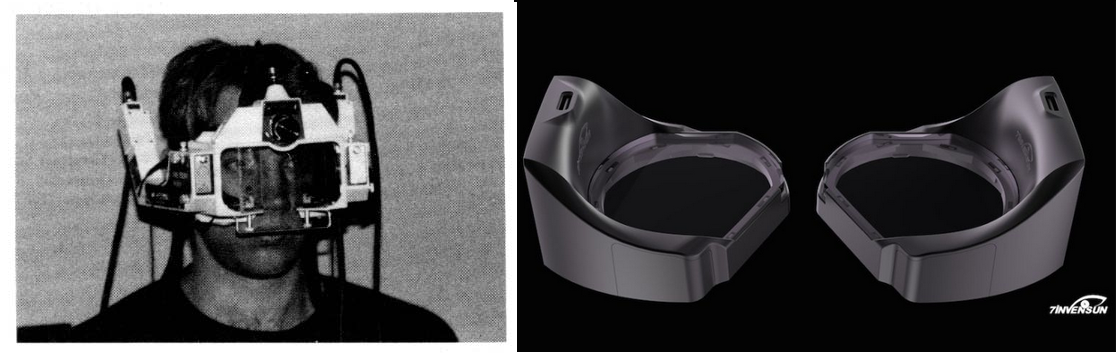
\psfig{file=7invensun_combo.png,width=3.3in}
\caption{Pictured left: \textit{NAC Eye Mark eye tracker} from the '80s. Pictured right: \textit{aGlass} eye tracker from 2017.~\cite{Levoy:Gaze}~\cite{Verge:Adi}}
\label{fig:fig3}
\end{figure}

\subsection{3D Rendering Concepts}
\label{sec:3dRendering}

\todo[inline, color=white]{This section will cover rendering concepts such as anti-aliasing (MSAA and FSAA), spatial/temporal artifacting, and possibly raytracing/pixel shading if space permits.}

\section{Foveated Renderer Design}
\label{sec:frDesign}
\todo[inline, color=white]{This section is most developed at the time of this writing.}
%peripheral blur, terrain tessellation, etc. 

When attempting to implement a foveated renderer to save on computational overhead, several factors must be considered. The goal of foveated rendering is to create graphical environments where the center of the user's gaze is directed at the portion of the screen rendered at the highest quality available, with resolution and level of detail progressively decreasing as retinal eccentricity increases.

The concept of multi-resolutional displays utilizing gaze tracking in their rendering algorithms has been around for decades, as evidenced by the work of Mark Levoy and Ross Whitaker in the 1980s~\cite{Levoy:Gaze}, however they were limited by the potential of their hardware as previously mentioned.

Perhaps the first notable work that actually claimed significant performance advantages in graphical rendering from this technology was that of Guenter et al. in 2012. This team  claimed that their renderer could produce results indistinguishable from full-resolution images, yet with around one fifth or sixth of the computational power previously required.

\subsection{Desktop Display Foveated Rendering (2012)}
\label{sec:microsoft}
Guenter et al. were attempting to validate previous research in the field by using what was cutting edge technology at the time to bridge the gap between theory and practice. Hardware had finally gotten to the point that they could take advantage of the work put forth by the likes of Levoy and Whitaker to make a renderer that capitalized on the opportunity for low cost optimization.

\subsubsection{Renderer Design Goals}
\label{mDesignGoals}
Guenter et al. aimed to obtain considerable speedup in processing capabilities while also avoiding any noticeable spatial or temporal artifacts. They conducted numerous user studies in order to verify that their system gave users difficulty in distinguishing between the foveated and non-foveated renders. The team also had to deal with a self-imposed constraint in that they wanted their solution to have the capacity to be retrofitted to improve existing applications. This meant that their anti-aliasing algorithm had to be effective while also requiring limited modification to shaders and geometry. They had to strike a fine balance between being specific enough to address their artifacting problem, while also being applicable to a range of applications~\cite{Guenter:Foveated}.

\subsubsection{Techniques Used}
\label{mTechniques}
In this instance, successful optimization depended on minimizing system latency, handling aliasing in the periphery, and finding the ideal balance of size and resolution for their eccentricity layers. They were able to reduce pixel shading by a factor of 10-15 due to their implementation of the following:

\begin{itemize}
\item MSAA: multisample anti-aliasing.
\item temporal jitter of the spatial sampling grid: the shifting back and forth of the eccentricity layer by 1/2 of its pixel pitch to reduce artifacting.
\item temporal reverse reprojection: blending of previous and current pixel values to increase the effective sampling.
\end{itemize}

Through numerous user studies and powerful optimization techniques, Guenter et al. became among the first developers to fully realize the potential of foveated rendering. However, it is worth noting that they were still limited by the technological constraints of their time:
\begin{quote}
Ideally, the graphics card would render at full display resolution
where the gaze is centered and continuously decrease resolution
outward from there. A more efficient method on current graphics
hardware is to approximate this ideal by rendering several overlapped 
rectangular regions called eccentricity layers.~\cite{Guenter:Foveated}
\end{quote}
This hardware-imposed weakness to their approach is one of the areas improved upon by subsequent efforts by other developers that built on their work. 

\begin{figure}
\centering
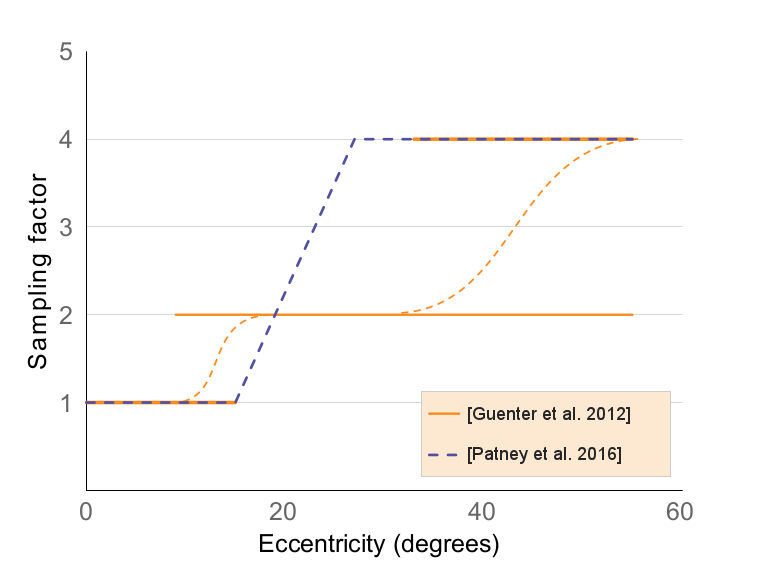
\psfig{file=sampling_eccentricity_Patney2.png,width =3in}
\caption{Comparison of sampling approaches by Patney et al. and Guenter et al.~\cite{Patney:Towards}}
\label{fig:fig4}
\end{figure}

\subsection{Virtual Reality Foveated Rendering (2016)}
\label{sec:nvidia}
Four years after the publication of \textit{Foveated 3D Graphics} by Guenter et al., eight developers from NVIDIA (Anjul Patney et. al.)  brought the technology of foveated rendering into virtual reality for a potentially important advance for the field. Guenter's team proposed that the true benefits of this rendering technology would be most apparent when the display had a larger field of view (FOV), and virtual reality head-mounted displays (HMDs) boast the largest FOV in any display to date: true 360\degree. Virtual reality is a perfect match for foveated rendering as many headsets already have gaze-tracking built in, so implementing these algorithms yields significant gain for very low cost.

Patney et al. set out to bring the speedup of foveated rendering to a field where the computational demand is rising and the size of the technology used is steadily shrinking. Any potential for increased computational power would have significant impact on the capabilities of VR.

\subsubsection{Renderer Design Goals}
\label{nDesignGoals}

Patney et al. specifically call out the aforementioned work from 2012 of Guenter et al.:

\begin{quote}
Prior foveated renderers like Guenter et al. [2012] \ldots focus on practical near-term techniques to reduce costs without explicitly identifying and minimizing perceptible artifacts introduced by foveation. Our studies show they often exhibit significant head- and gaze-dependent temporal aliasing, distracting users and breaking immersion.~\cite{Patney:Towards}
\end{quote}

Having specified weaknesses in previous approaches, the developers at NVIDIA worked to find new methods that would minimize temporal aliasing and any ``tunnel vision''-like sensation. To this end, they prioritize the preservation of contrast, as their user studies suggest that enhancing contrast negates the effects of tunnel vision, only perceiving visual stimuli from the central field of view, caused by the reduction in peripheral detail.

\subsubsection{Techniques Used}
\label{nTechniques}

Patney et al. built directly on the existing work of others by adding parameter tweaks and supplementary algorithms. For example, rather than render three foveal layers like the approach of the Guenteer et al., Patney et al. utilize a piecewise linear variation of shading rate in a single layer. This alternate approach enables them to transition to a lower level of detail at smaller retinal eccentricities, leading to more peripheral pixels and more computational speedup (see \textbf{Figure~\ref{fig:fig2}}). Additionally, they differ from other approaches in that they sample visibility at full resolution throughout the entire image rather than sampling at multiple resolutions. They instead lower detail levels by varying the pixel shading rate. This decision ended up requiring them to use a new post-processing anti-aliasing algorithm, variance sampling, to improve visual fidelity.

\subsubsection{Variance Sampling}
\label{variance}

\todo[inline, color=white]{This section will cover the implementation of Variance Sampling by Patney et al. in their foveated renderer design.}

\subsubsection{Perceptual Visual Target}
\label{visualTarget}
Patney et al. differ further in their design process from some of their predecessors in that they used something they referred to as a Perceptual Visual Target to guide the design~\cite{Patney:Towards}. Essentially, their design team created a demonstrational model of sorts that emulated their ideal version of foveated rendering using preprocessed scenes. They then tested this demo by conducting user studies to confirm that their intended optimizations would be effective. Once they had a user-approved renderer emulation, they began the design process with the goal of being able to render what was shown in the perceptual visual target, albeit in real time. 

This process of guiding their development lead to impressive overall user satisfaction, with their renderer yielding superior results in a number of facets.
\todo[inline, color=white]{This will be elaborated on in the subsequent section: Results. I plan on discussing user studies there, so this is a placeholder transition.}


\iffalse
\begin{figure}
\centering
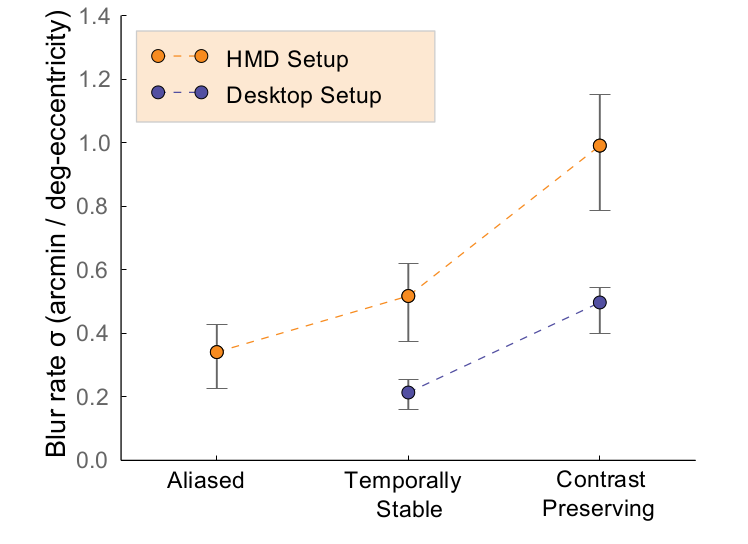
\psfig{file=frMethods_Patney.png,width =3in}
\caption{Comparison of different foveation techniques by Patney et al. in their studies on what threshold of blur rate their users couldn't detect.~\cite{Patney:Towards}}
\label{fig:fig3}
\end{figure}


\begin{figure}
\centering
\psfig{file=sampling_eccentricity_Patney.png,width =3in}
\caption{Comparison of sampling approaches by patney et al. and Guenter et al.~\cite{Patney:Towards}}
\label{fig:fig2}
\end{figure}


\begin{figure}
\centering
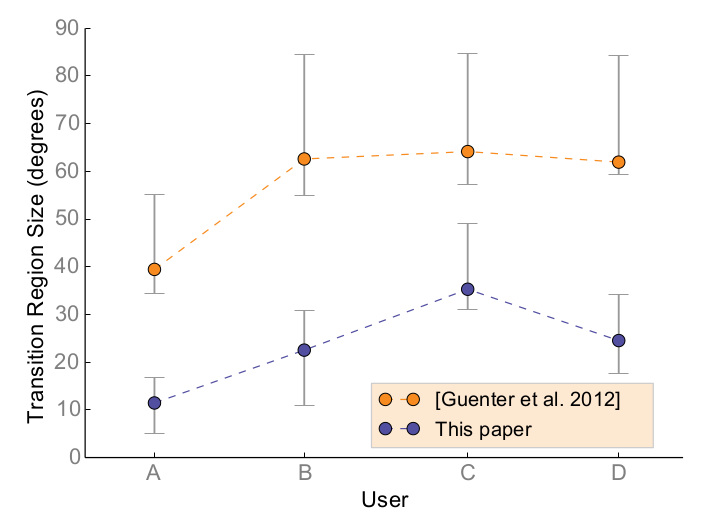
\psfig{file=transition_region_Patney.png,width =3in}
\caption{Comparison Transition Region Size for Guenter et al. and Patney et al. In this instance, having a lower threshold is ideal because that allows more peripheral pixels to be shaded, reducing computational overhead.~\cite{Patney:Towards}}
\label{fig:fig4}
\end{figure}
\fi


\section{Results}
\label{sec:results}

Outline Notes: This section will summarize what rendering setups users said worked best in the numerous studies I have found, and also will highlight what seemed to not work so good. So far it seems that contrast-preserving temporally stable foveation is one of the most effective methods. Essentially by the end of this section the audience should have a sense of what variables makes foveated rendering effective, why this is, and how satisfied users currently are with the experience.

\section{Conclusion}
\label{sec:conclusion}
Outline Notes: Restate the most effective techniques from section three and what gains this technology yields, set the tone for the cutting edge of this field as work continues. Maybe discuss some other impacts foveated rendering has had; there was one paper I found: GazeSim: simulating foveated rendering using depth in eye gaze for VR, that discussed how technology like this was used to reduce user nausea in VR by streamlining the rendering process by using all of their resources to give a higher quality to wherever the user was looking, which led to less latency and a more enjoyable experience. Something like this advance would be a good way to once again relate the topic to common user experiences and demonstrate the effectiveness and exciting path this technology is taking.

\section{Acknowledgements}
\label{sec:acknowledgments}

\bibliographystyle{abbrv}

\bibliography{frvr_paper}  

\end{document}
